% Toolbar icon: edges — iso cube, uniformly shaded, with its silhouette and the three
% visible interior edges over-stroked; reads as 'faces with edges emphasised'.
% Same vertex layout as wireframe.tex/addBox.tex. Distinct from wireframe.tex
% (unfilled + dashed hidden edges) and volume.tex (per-face shading, thin edges).
\documentclass[tikz,border=2mm]{standalone}
\usetikzlibrary{arrows.meta,calc,shapes.geometric}
\begin{document}
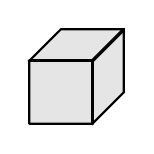
\begin{tikzpicture}[line width=1.3pt, line cap=round, line join=round, >=Stealth, x=1mm,y=1mm]
  \draw[thick, fill=gray!20] (-6,-8) -- (2,-8) -- (6,-4) -- (6,4) -- (-2,4) -- (-6,0) -- cycle;
  \draw[very thick] (-6,0) -- (2,0) -- (2,-8);
  \draw[very thick] (2,0) -- (6,4);
\end{tikzpicture}
\end{document}
